\chapter{Fault Detection and Diagnosis with Offline Processing}


The test system used for this project is the Condition Monitoring Laboratory (CML) in the national Centre for Advanced Tribology at Southampton (nCATS).
This system was developed to demonstrate the principle of condition monitoring through vibration analysis and is the result of several individual projects, group projects and summer internships (Fig \ref{fig:CMrig}).
It performs data collection, transfers to the frequency domain and calculates a rolling average of vibration RMS online.
The basic setup is a motor with a shaft which is supported by three rolling element bearings.
Each of the bearings has a piezoelectric accelerometer mounted on it with a screw thread \cite{CMlab}.
The middle bearing is mounted on a platform which can be pushed with a linear actuator to induce bending in the shaft.
Some of the bending is absorbed by the coupling between the shaft and the motor which is flexible to allow quick assembly of the CML without the need for precise mountings.
The bearings also have spherical casings within their pillow housings.
Therefore while the linear actuator can be controlled to provide a force to the platform, exact calibration is not possible.
\par

Using the CML in its existing setup provided two main advantages for the project:
\begin{itemize}
    \item Compare the performance of the the embedded CMS to more sophisticated hardware and software
    \item Test the ability of simple statistics to identify the condition of the machine with a sophisticated data collection system
\end{itemize}

\begin{figure}
    \centering
    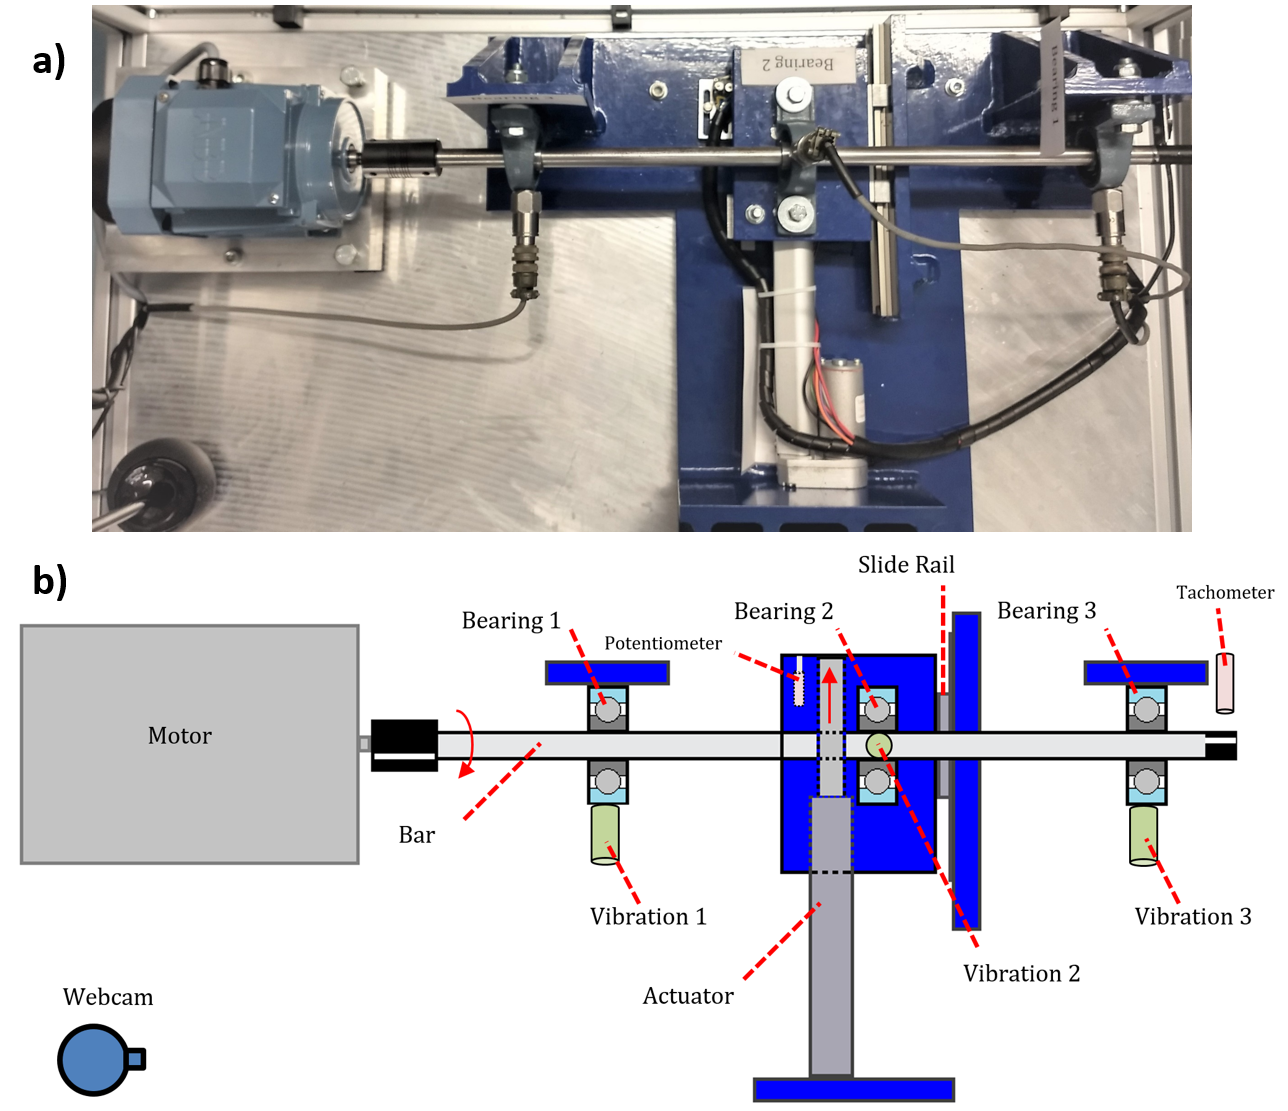
\includegraphics[width=\linewidth]{ConditionMonitoringRig.PNG}
    \caption{CML in nCATS Laboratory - a) Photo, b) Diagram (Reproduced from \cite{CMlab})}
    \label{fig:CMrig}
\end{figure}

\section{Condition Monitoring Laboratory}

The motor is a 3-phase squirrel cage induction motor with 4 poles, power consumption of 0.18 kW and runs at up to 1500 rpm \cite{CMlab_motor}.
Acceleration is measured on each bearing with Omega ACC786A accelerometers, which have a bandwidth of 14 kHz, sensitivity of 100 mV/g within a range of $\pm$80 g, resonant frequency at 30 kHz and is surrounded in an industrial casing \cite{CMlab_accelerometer}.
Data is collected at 5 kHz using National Instruments Data Acquisition Cards and sent to a PC for storage and processing.
Motor speed is verified with a light-based tachometer.

\section{Experimental Methodology}

As the CML has been in use for several years, it is unlikely that it is in a completely healthy condition.
To ensure a healthy condition for baseline measurements, new bearings will be fitted and the shaft will be aligned carefully to reduce any bending.
Data will be collected from all three accelerometers for processing.
Next, bending will be induced in the shaft.
Finally, the shaft will be returned to the healthy condition, and bearing 3 will be replaced with an older bearing which is thought to have damage.
This bearing will be inspected after all experimentation has finished as the inspection process is destructive.
\par

By collecting information about the vibration at each bearing in three different conditions, processing of the data should reveal significant differences in statistics extracted from the frequency spectrum, as shown by Moosavian et al. \cite{VIB_moosavian}.
The time data will also be compared to the ISO bearing damage chart \cite{ISO13373-3}.
The viability of the CML and individual accelerometer mounting points for further testing can then be assessed.
\par

Acceleration data was sampled at 5 kHz for 5 seconds, and each condition was sampled 10 times.
The sampling rate cannot be altered through the existing software.
Each sample was transformed to the frequency domain before the maximum, RMS and STD of the frequency spectrum were extracted.
The average values of these statistics were also calculated across the samples.
The frequency spectrums were then averaged to remove transient signals.
\par

The nCATS laboratory is busy and other experiments were taking place during testing. 
Therefore it is possible that some noise was introduced to the results from outside sources. 
However, given that the purpose of this project is to implement condition monitoring on a ship, an incredibly noisy environment, any techniques used should show resilience to noise \cite{CBM_lr}.

\section{Results}

It is clear that the three conditions inspected have distinct vibrational signatures (Fig \ref{fig:PP1}).
These signatures also vary significantly on each of the different bearings. 
These results support the use of these statistical features for fault detection.
Looking at only the values of maximum and STD, there is almost no overlap between the conditions, and simple inequalities are sufficient to classify them (Fig \ref{fig:PP2}).
The similarities to the results used for training of a neuro-fuzzy inference model suggest that the CML will be suitable for testing the embedded system and could provide a dataset for ANNs or ML models in the future \cite{VIB_moosavian}.
\par

Closer inspection of the time data revealed that a significant DC component was affecting the results, particularly of Bearing 1 and Bearing 3.
A DC component would result from gravity if not processed properly.
It is possible that the software in the existing setup did not account for this component or that it resulted from imperfect fitting or calibration of the accelerometer.
Fig \ref{fig:PP5} shows the results following extraction of this component by subtracting the mean value from each sample in the time domain.
The maximum is affected as the largest component often was the DC component, which was not significantly affected by the changing condition.
After removal, the maximum is closely related to the condition of the machine.
\par

Bearing 2 provides the most clearly separated data.
This was expected in the case of bending, as the bending force travels directly through the bearing, but it also detects the effect of the faulty bearing. 
As such, this bearing is most suitable for further investigation.
The averaged frequency spectrum of Bearing 2 in the different conditions reveals significant differences (Fig \ref{fig:PP4}).
Although values were calculated up to 2.5 kHz, there is nothing of interest beyond the range shown.
The rotor frequency and its harmonics are visible for all conditions.
With bending, the rotor frequency is diminished and its second and third harmonics are larger, as expected (Table \ref{tab:vibfaults}).
There is also more noise below 500 Hz.
The faulty bearing signal is differentiated by a largely increased maximum at the rotor frequency.
This could be result of loose housing on the bearing.
The rotor harmonics are also less distinct.
All three conditions show a small peak at approximately 1160 Hz, which shifts to a slightly lower frequency under bending. The cause of this peak is not yet known, although it may be related to bearing pass frequencies.
\par

Comparing the results to the chart of bearing fault severity provided by the ISO, the expected results are not seen (Fig \ref{fig:PP6}).
Firstly, the chart had to be extrapolated to lower values of acceleration to accommodate the measured values.
Bearing 1 is still below these limits so is discounted.
Bearing 2 and Bearing 3 both show separation in values between the conditions.
However, the supposed bearing fault condition appears to be healthier than the healthy condition.
With Bearing 2, the bent condition is on the border of the alarm values for a bearing fault.
This suggests that the bearing is damaged as thought, and that there may be some issues with using the existing system to diagnose faults.
Nevertheless, values from the time domain can be used to classify the conditions effectively.
\par

This experiment validates the CML for testing of the embedded system.
Bearing 2 has the most distinct vibration signatures so will be used for accelerometer mounting.


\begin{figure}
    \centering
    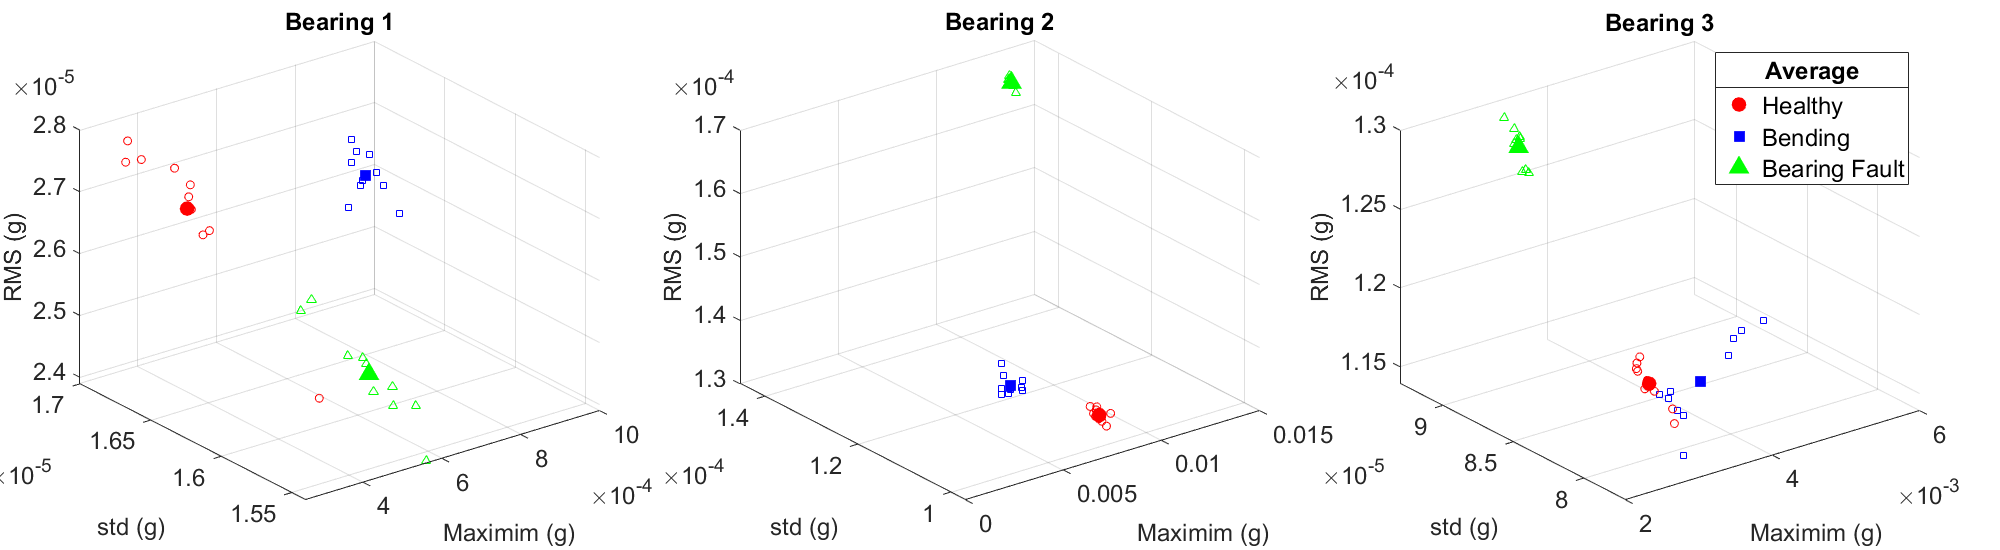
\includegraphics[width=\linewidth]{PreProcessing1.png}
    \caption{Results from investigation of existing condition monitoring setup}
    \label{fig:PP1}
\end{figure}

\begin{figure}
    \centering
    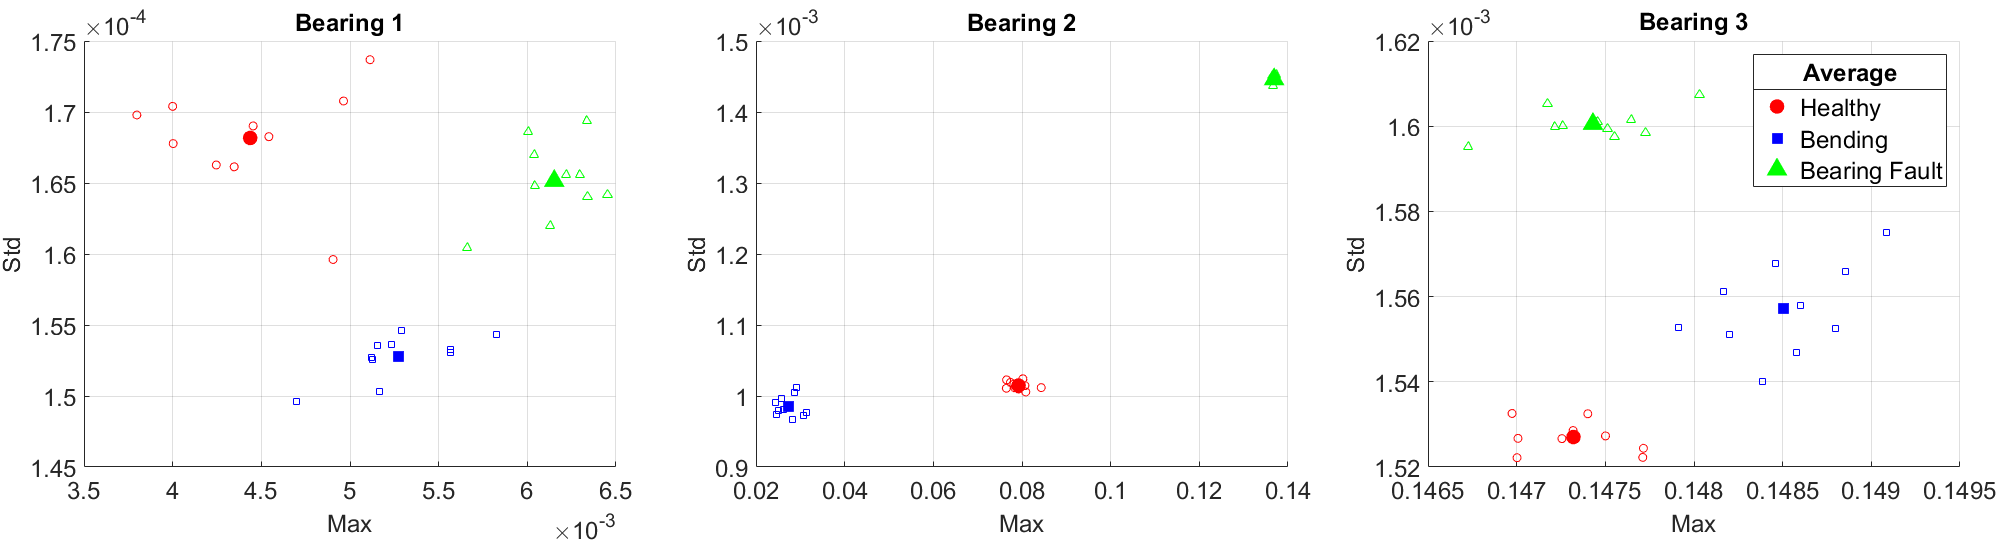
\includegraphics[width=\linewidth]{PreProcessing2.png}
    \caption{Results from investigation of existing condition monitoring setup with only maximum and standard deviation of the frequency spectrum shown}
    \label{fig:PP2}
\end{figure}

\begin{figure}
    \centering
    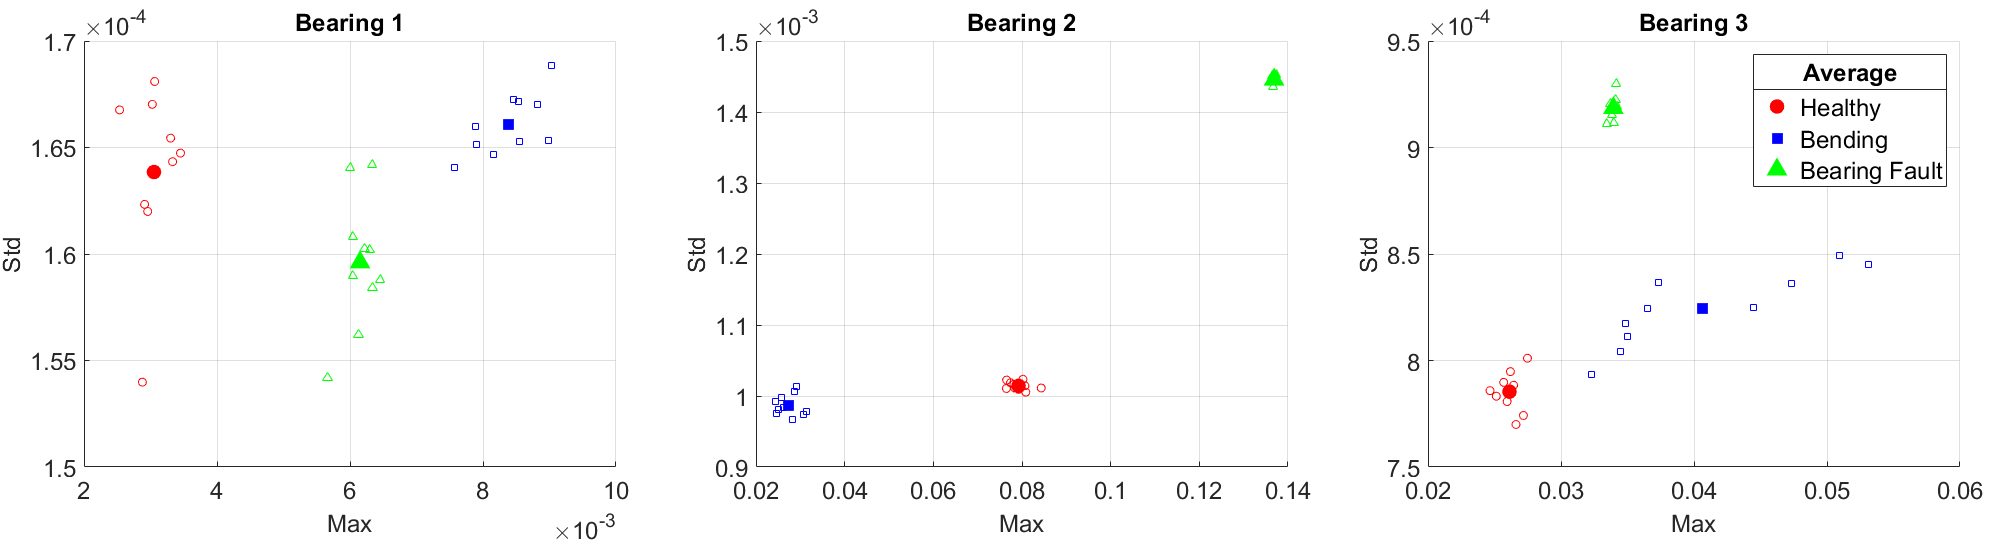
\includegraphics[width=\linewidth]{PreProcessing5.png}
    \caption{Results shown after removing DC frequency component}
    \label{fig:PP5}
\end{figure}

\begin{figure}
    \centering
    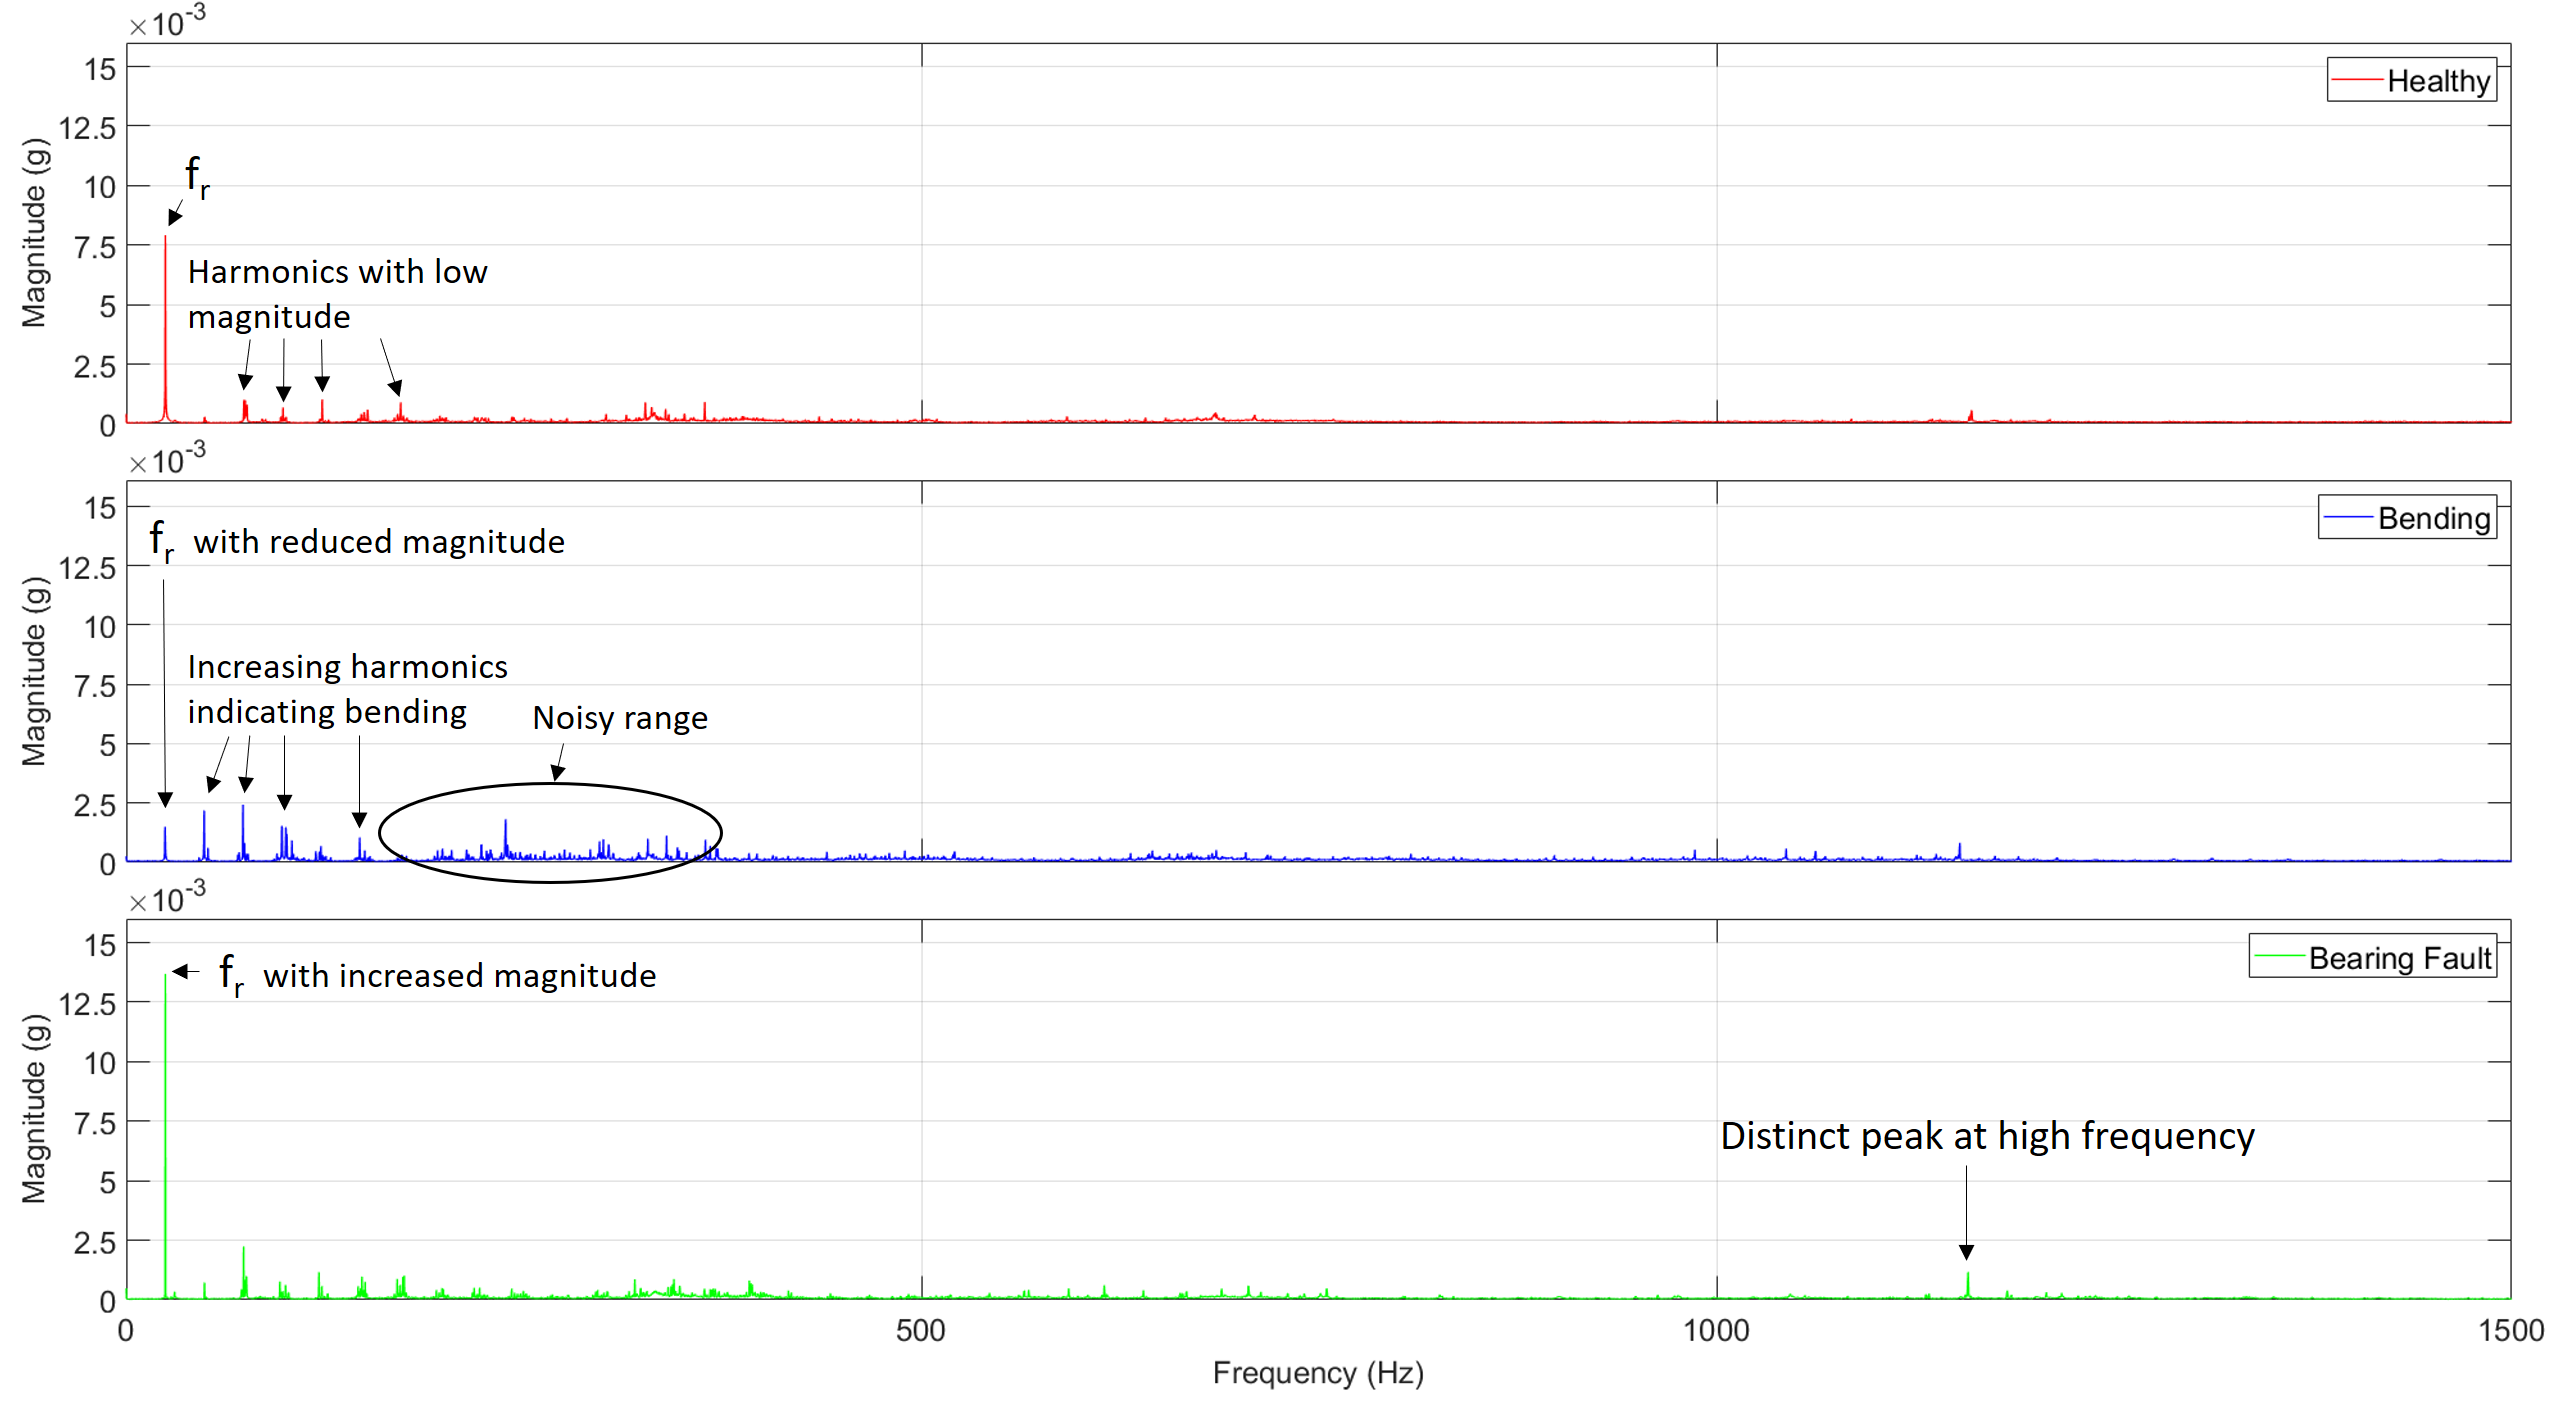
\includegraphics[width=\linewidth]{PreProcessing4.PNG}
    \caption{Averaged frequency spectrum for Bearing 2 of CML with annotations}
    \label{fig:PP4}
\end{figure}

\begin{figure}
    \centering
    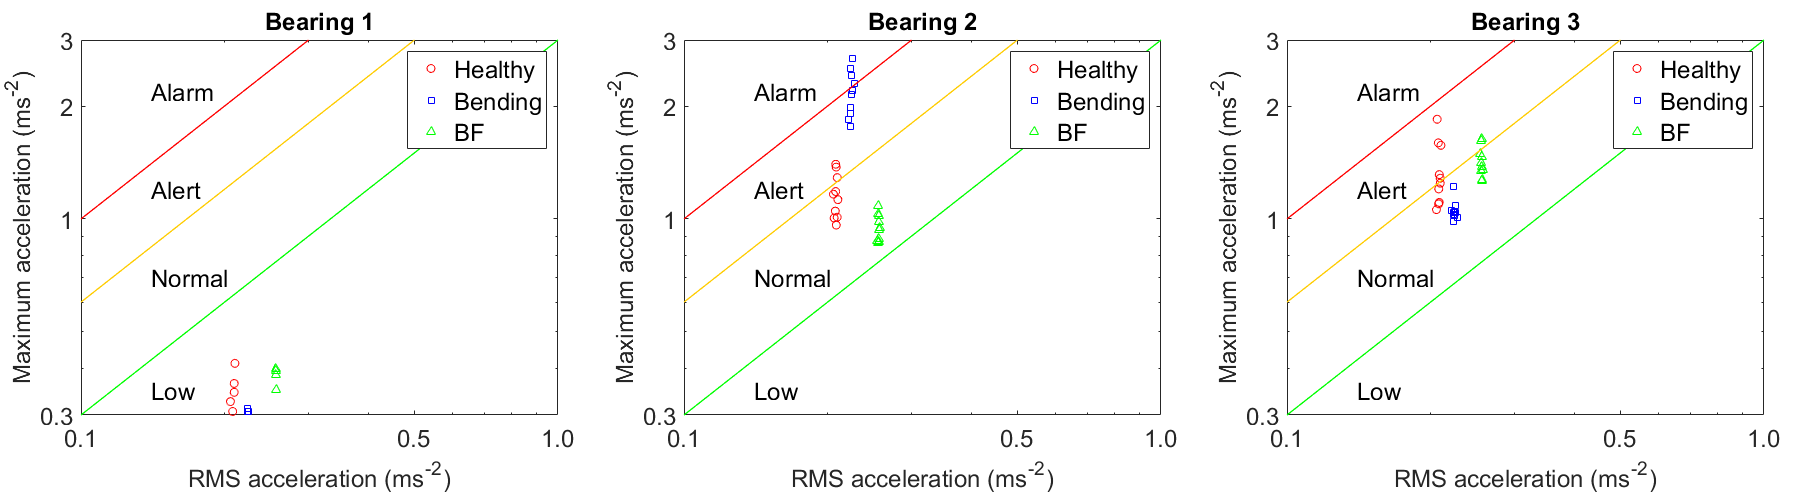
\includegraphics[width=\linewidth]{PreProcessing6.png}
    \caption{Comparison of results with ISO bearing fault chart}
    \label{fig:PP6}
\end{figure}

\section{Evaluation}

While the results from this experiment will be helpful to the development of the embedded system, there are some notes regarding the use of the CML.
It proved very difficult to replace the bearings due to the way the CML has been built.
Small variations in the position of the bearings results in bending and it is difficult to exactly replicate the healthy conditions.
The linear actuator control needs to be improved in the future to allow for finer and more repeatable control.
This follows suggestions that it be replaced by a stepper motor \cite{CMlab}.
The entire CML is mounted loosely on a heavy metal top.
It should be fixed in place to prevent small movements of the bearing base or motor.